\chapter{ВЫБОР ФИЗИЧЕСКИХ ПАРАМЕТРОВ СКАНЕРА}
    \section{Выбор метода сканирования}
        Для выбора метода сканирования необходимо определить условия работы и ограничения накладываемые существующей конструкцией прототипа на модуль сканирования и сопоставить их с требованиями и особенностями методов измерения, а также учесть требования технического задания.
        
        Поскольку все методы оптические, они предъявляют требования к освещённости окружения. Освещение рабочего поля должно быть равномерным, не слишком ярким и не должно вызывать бликов. При этом сканируемые поверхности не должны быть зеркальными или поглощающими свет.
        
        Параметры конструкции прототипа:
        \begin{itemize}
            \item габариты корпуса $ 400 \times 550 \times 560 \text{ мм} $
            \item размеры рабочей области $ 200 \times 200 \text{ мм} $
            \item контролируемое освещение
            \item закрытый корпус
        \end{itemize}
        
        Видно, что свободное пространство в принтере ограничено из-за наличия подвижного печатающего узла, габариты которого выходят за пределы рабочей зоны. Таким образом становится невозможно использование крупных компонентов в разрабатываемой системе сканирования.

        Поэтому метод структурированного света в данном случае не подходит, так как требует использования проектора, который имеет большие размеры и высокую стоимость. Существуют и миниатюрные проекторы, однако их стоимость ещё выше. Алгоритмы используемые в методе структурированного света являются сложными, что увеличивает требования к вычислительными мощностям прототипа и как следствие его стоимость.

        Лазерная триангуляция накладывает дополнительные ограничения на возможные сканируемые поверхности, так как использует видимое излучение для работы. Это значит, что сканирование предметов такого-же цвета, что и свет излучаемый лазером, будет сильно затруднено. Такая ситуация может возникнуть, если изделие, например торт, будет обладать цветным покрытием. Однако это можно преодолеть если использовать сканирование в темноте. Это позволит сканировать такие объекты, тем не менее качество таких сканов будет хуже из-за явления самозасветки лазера.
        Так же, используя этот метод, модуль целиком или только лазер, необходимо перемещать вдоль сцены, чтобы захватить все профили исследуемой поверхности. Это снизит скорость сканирования в сравнении с остальными методами.
        Однако для реализации этого метода достаточно одной камеры и лазерного модуля, которые можно расположить компактно. Также это снижает стоимость прототипа, что важно в данном проекте.

        Метод фотограмметрии или стереозрения в данной работе не рассматривается, так как этот метод был опробован ранее и не показал удовлетворительных результатов. В данном методе теряется большое количество данных сцены и точность оставляет желать лучшего. При этом для этого необходимы две камеры, что так же проблематично встроить в существующую систему\cite{SkripkoPASEKA}.
        
    \section{Выбор компоновки}
        Общий план модуля сканирования представлен на рисунке \ref{pic:general_view} (подвижный узел не показан). Он демонстрирует относительное расположение элементов в пространстве. В данной компоновке лазер направлен перпендикулярно столу (параллельно оси $ Z $), линия проекции лазера параллельна оси $ Y $ стола, а камера под углом к вертикали не имея поворота относительно остальных осей. Движение модуля происходит параллельно оси $ X $ системы координат принтера в сторону уменьшения координаты.

        \begin{figure}[H]
            \centering
            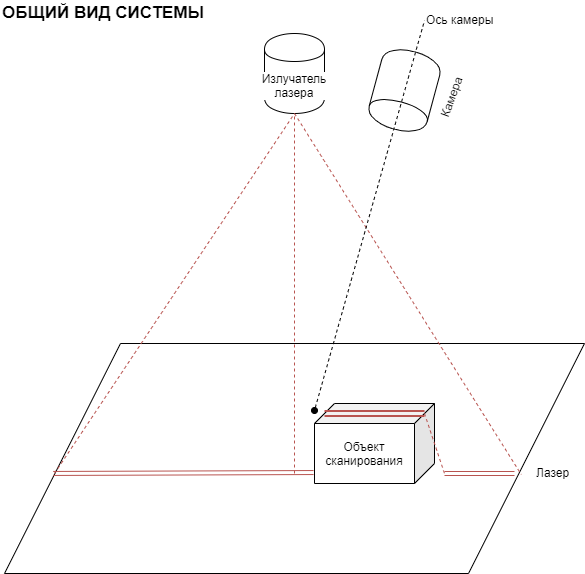
\includegraphics[width=0.5\linewidth]{general_view}
            \caption{Общий план модуля}
            \label{pic:general_view}
        \end{figure}

        Для обеспечения лучших показателей точности необходимо выбрать расстояние и угол между оптической осью камеры и осью лазера, а так же расстояние от камеры до стола. Этот этап важен, так как от этих параметров зависит разрешающая способность сканера и видимая рабочая зона. Чем ниже камера к столу, тем меньше дискретизация значений координат, но одновременно меньше видимая область. Угол наклона камеры также влияет на дискретизацию и видимую область сканера.
        С помощью расчётов, приведённых в разделе \ref{sec:error} были установлены следующие величины этих размеров:
        \begin{table}[H]
            \centering
            \caption{Основные размеры модуля сканирования}\label{table:dims}
            \begin{tabular}{|l|c|} \hline
                Высота над столом& $ 140  \pm 10 \text{ мм} $\\ \hline
                Расстояние от камеры до лазера& $ 140  \pm 10 \text{ мм} $\\ \hline
                Угол между осями камеры и лазера& $ 45 \pm 15\degs $\\ \hline
            \end{tabular}
        \end{table}
        Данные величины позволяют достичь необходимой по ТЗ точности в $ \pm 0.5 \text{ мм} $ и ширины обзора 200 мм.
        Для модуля используется камера Microsoft Lifecam Cinema с максимальным разрешением $ 1280 
        \times 720 $ и максимальной частотой 30 кадров в секунду. Использование данной камеры позволяет упростить процесс калибровки, так как она обладает встроенной ректификацией изображения. Лазерный модуль S-2S с толщиной проецируемой линии в 3 мм. Точность измерений находится в обратной зависимости от толщины линии лазера.

        Камера устанавливается в специальный держатель, в котором предусмотрена калибровка поворота камеры для более точного направления на интересующую зону и надёжного закрепления. Реализация крепления и установки модуля в систему рассматривается в работе\cite{matsu}. 

        К конструкции модуля предъявляются следующие требования:
        \begin{itemize}
            \item минимизация влияния вибрации на положение камеры
            \item размеры в пределах указанных в таблице \ref{table:dims}
            \item допускаются посторонние объекты в верхней половине кадра занимающие не более четверти высоты кадра
            \item возможность калибровки поворота камеры
            \item возможность калибровки поворота лазера
        \end{itemize}
    
        Итоговый вид модуля в составе прототипа изображён на рисунке \ref{pic:final_model}. Крепление камеры изображено на рисунке \ref{pic:camera_mount}.

        \begin{figure}[H]
            \centering
            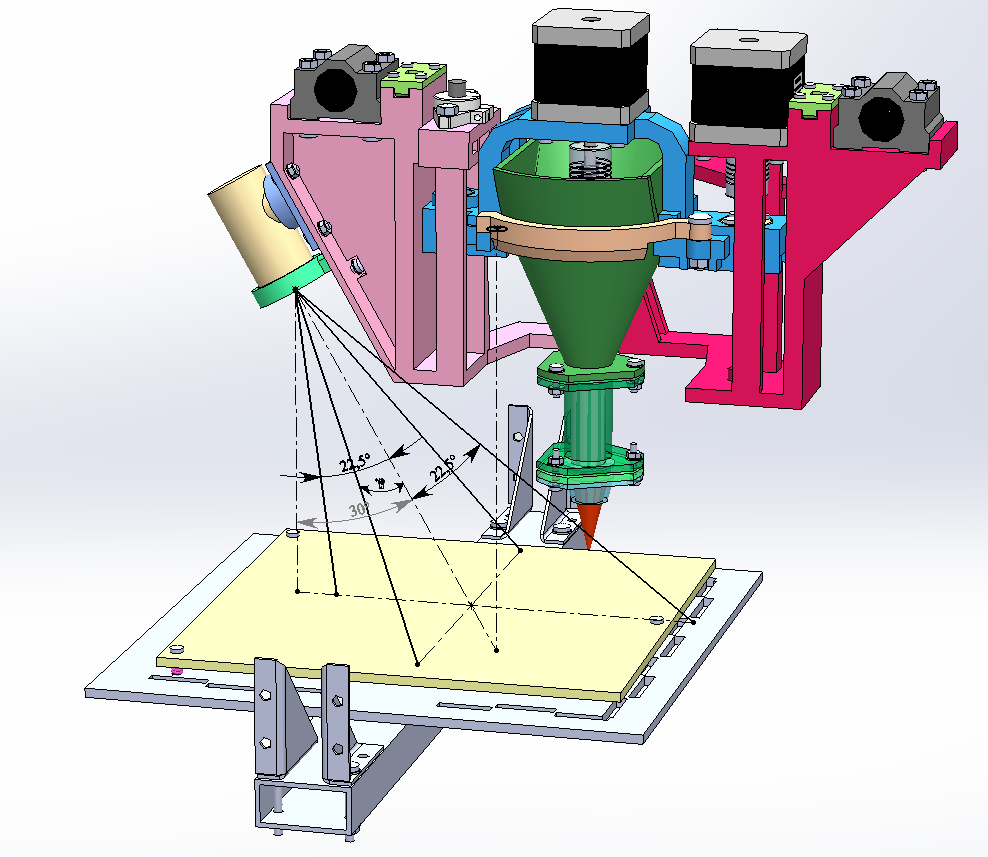
\includegraphics[width=\linewidth]{final_model_camera_view}
            \caption{Общий вид в принтере}
            \label{pic:final_model_camera_view}
        \end{figure}
        
        \begin{figure}[H]
            \centering
            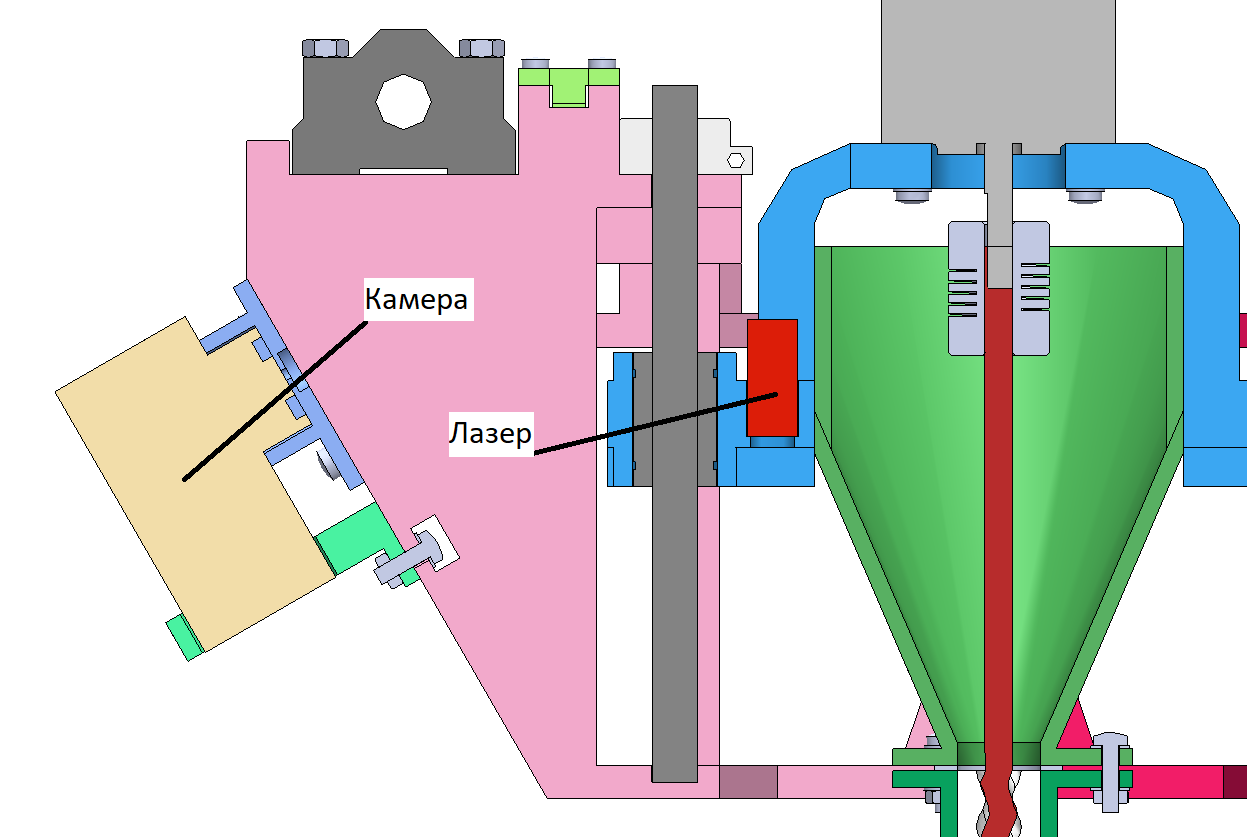
\includegraphics[width=\linewidth]{final_model_capts}
            \caption{Финальная компоновка модуля сканирования}
            \label{pic:final_model}
        \end{figure}
    
        \begin{figure}[H]
            \centering
            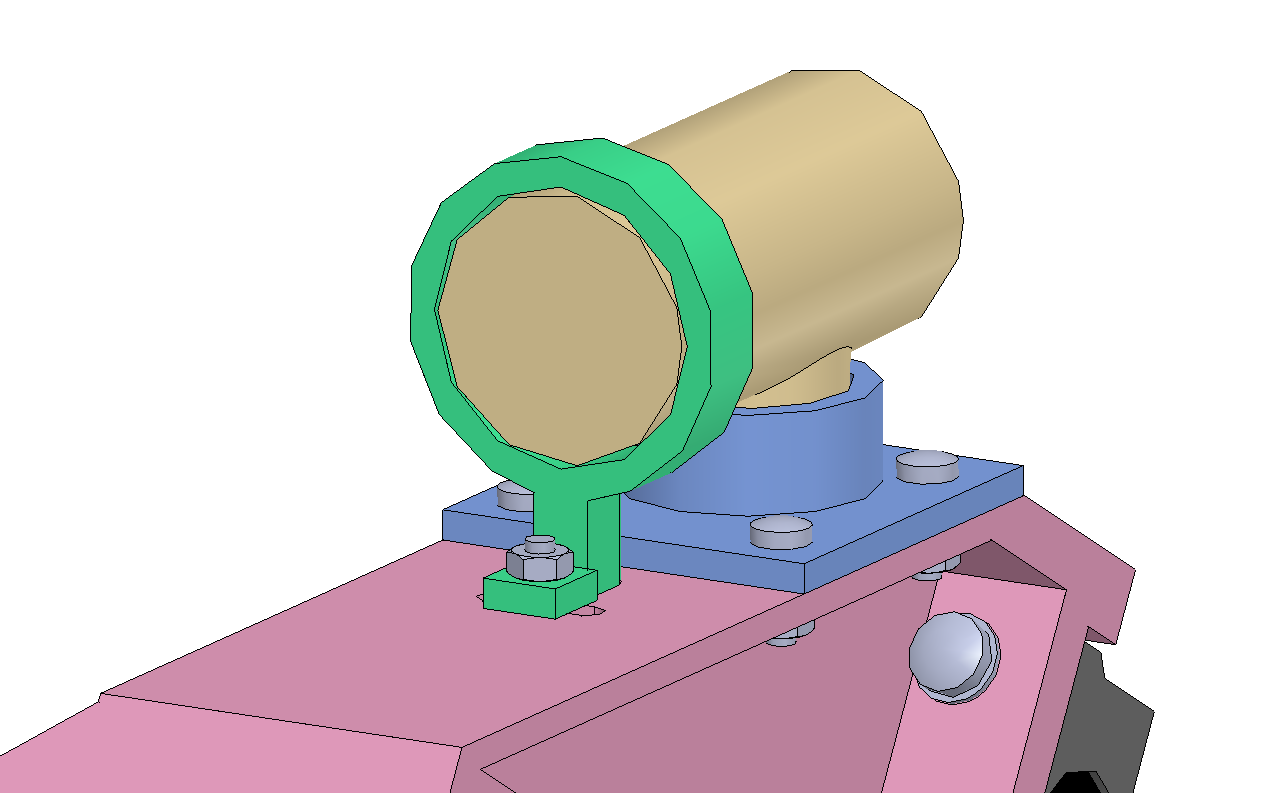
\includegraphics[width=0.5\linewidth]{camera_mount}
            \caption{Крепление камеры}
            \label{pic:camera_mount}
        \end{figure}